\documentclass[11pt,aspectratio=169]{beamer}
% Versión handout (sin transiciones): descomentar y comentar la línea anterior.
% \documentclass[handout,11pt,aspectratio=169]{beamer}
\usepackage[utf8]{inputenc}
\usepackage[T1]{fontenc}
\usepackage[spanish]{babel}
\usepackage{pgfpages}
\usepackage{fancyvrb}
\usepackage{tikz}
\usepackage{pgfplots}
\usepackage{soul}
\usepackage{booktabs}
\usepackage{amsmath}
\usepackage{amssymb}
\usepackage{hyperref}
\usepackage{listings}
\usepackage{xcolor}
\usepackage{graphicx}
\usepackage{array}

\pgfplotsset{compat=1.18}
\usetikzlibrary{arrows.meta,positioning,shapes.geometric,fit,backgrounds,calc,shadows.blur}

% COLORES
\definecolor{blue}{RGB}{0,118,186}
\definecolor{red}{RGB}{181,23,0}
\definecolor{gray}{RGB}{146,146,146}
\definecolor{lightblue}{RGB}{235,244,250}

\definecolor{gray97}{gray}{.97}
\definecolor{gray75}{gray}{.75}
\definecolor{gray45}{gray}{.45}

\lstset{
     frame=Ltb,
     backgroundcolor=\color{gray97},
     basicstyle=\tiny\ttfamily,
     commentstyle=\color{gray45},
     breaklines=true,
     showstringspaces=false,
     columns=fullflexible,
     keepspaces=true,
     literate={á}{{\'a}}1 {é}{{\'e}}1 {í}{{\'i}}1 {ó}{{\'o}}1 {ú}{{\'u}}1 {Á}{{\'A}}1 {É}{{\'E}}1 {Í}{{\'I}}1 {Ó}{{\'O}}1 {Ú}{{\'U}}1 {ñ}{{\~n}}1 {Ñ}{{\~N}}1 {ü}{{\"u}}1 {¿}{{?`}}1 {¡}{{!`}}1,
}

\usetheme{auriga}
\usecolortheme{auriga}

\newcommand{\todo}{\textcolor{red}{\textbf{TODO(alumno)}}}
\newcommand{\code}[1]{\texttt{#1}}

\title{\Large{Laboratorio 02: Gemini, JSON y vault Obsidian\\ \normalsize De texto limpio a conocimiento navegable}}
\subtitle{Recuento del lab 01, extracción LLM, validación JSON y persistencia Markdown}
\author{Dr. Juan Bekios Calfa}
\institute[UCN]{\textbf{Machine Learning / Gestión de Proyectos en IA}\\Universidad Católica del Norte}
\date{\textbf{Publicación:} Septiembre 2026 \hspace{1cm} \textbf{Entrega:} Por definir}

\begin{document}

\begin{frame}
\titlepage
\end{frame}

%------------------------------------------------
\begin{frame}{Qué cambia en esta segunda parte}
\begin{columns}[T,onlytextwidth]
\column{0.58\textwidth}
\footnotesize
\begin{itemize}[<+->]
\item El laboratorio 01 dejó un corpus: URLs, HTML y texto limpio.
\item Ahora Gemini transforma ese texto en JSON con el contrato del curso.
\item El código de extracción es \textbf{simple y ejecutable}: el alumno debe mejorarlo.
\item El vault de Obsidian sigue siendo \todo{}: el alumno genera la jerarquía Markdown.
\end{itemize}
\column{0.38\textwidth}
\centering
\resizebox{!}{0.62\textheight}{%
\begin{tikzpicture}[font=\scriptsize, node distance=0.48cm]
\node[draw=blue, fill=lightblue, rounded corners=2mm, minimum width=2.7cm, minimum height=0.55cm, align=center] (a) {Lab 01: captura};
\node[draw=blue, fill=lightblue, rounded corners=2mm, minimum width=2.7cm, minimum height=0.55cm, below=of a, align=center] (b) {Texto limpio};
\node[draw=blue, fill=lightblue, rounded corners=2mm, minimum width=2.7cm, minimum height=0.55cm, below=of b, align=center] (c) {Gemini + JSON};
\node[draw=red, fill=red!10, rounded corners=2mm, minimum width=2.7cm, minimum height=0.55cm, below=of c, align=center] (d) {Obsidian};
\draw[-{Latex[length=1.6mm]}, thick, blue] (a)--(b);
\draw[-{Latex[length=1.6mm]}, thick, blue] (b)--(c);
\draw[-{Latex[length=1.8mm]}, thick, red] (c)--(d);
\end{tikzpicture}%
}
\end{columns}
\end{frame}

%================================================
\section{Recuento del laboratorio 01}

%------------------------------------------------
\begin{frame}{Idea central (laboratorio 01)}
\small
\begin{block}{Pregunta de trabajo}
¿Cómo transformar noticias delictuales publicadas en Internet en una base de conocimiento estructurada que permita identificar hechos, entidades y relaciones?
\end{block}

\vspace{0.2cm}
\begin{itemize}
\item No se entrena clustering: los grupos nacen de entidades compartidas.
\item No se usa una base de datos tradicional como persistencia final.
\item El identificador \code{id\_noticia} recorre todo el flujo: HTML $\rightarrow$ texto $\rightarrow$ JSON $\rightarrow$ nota Markdown.
\end{itemize}
\end{frame}

%------------------------------------------------
\begin{frame}{Arquitectura: qué ya corre y qué falta}
\centering
\resizebox{0.96\linewidth}{!}{%
\begin{tikzpicture}[font=\tiny, node distance=0.55cm,
box/.style={draw=blue, fill=lightblue, rounded corners=2mm, minimum width=2.05cm, minimum height=0.62cm, align=center},
rbox/.style={draw=red, fill=red!10, rounded corners=2mm, minimum width=2.05cm, minimum height=0.62cm, align=center},
arrow/.style={-{Latex[length=1.7mm]}, thick}]
\node[box] (a) {Internet\\Google News};
\node[box, right=0.55cm of a] (b) {URLs\\seleccionadas};
\node[box, right=0.55cm of b] (c) {Captura\\HTML/texto};
\node[box, right=0.55cm of c] (d) {Limpieza\\normalización};
\node[box, below=0.85cm of d] (e) {Gemini\\LLM};
\node[box, left=0.55cm of e] (f) {JSON\\validado};
\node[rbox, left=0.55cm of f] (g) {Markdown\\automático};
\node[rbox, left=0.55cm of g] (h) {Vault\\Obsidian};
\draw[arrow, blue] (a)--(b);
\draw[arrow, blue] (b)--(c);
\draw[arrow, blue] (c)--(d);
\draw[arrow, blue] (d)--(e);
\draw[arrow, blue] (e)--(f);
\draw[arrow, red] (f)--(g);
\draw[arrow, red] (g)--(h);
\end{tikzpicture}%
}

\vspace{0.25cm}
\footnotesize
Azul: implementado (lab 01 + extracción de este lab). Rojo: \todo{} Obsidian y análisis.
\end{frame}

%------------------------------------------------
\begin{frame}{CRISP-DM adaptado}
\begin{columns}[T,onlytextwidth]
\column{0.55\textwidth}
\scriptsize
\begin{enumerate}
\item Comprensión del negocio.
\item Comprensión de los datos.
\item Preparación (captura y limpieza).
\item Extracción con Gemini.
\item Validación del JSON.
\item Generación de conocimiento en Obsidian.
\item Evaluación y análisis crítico.
\end{enumerate}
\vspace{0.15cm}
\begin{block}{En este laboratorio}
Se implementan los pasos 4 y 5. El paso 6 lo completa el alumno.
\end{block}
\column{0.42\textwidth}
\centering
\resizebox{\linewidth}{!}{%
\begin{tikzpicture}[font=\tiny, every node/.style={align=center}]
\node[draw=blue, fill=lightblue, rounded corners=2mm, minimum width=2.0cm, minimum height=0.58cm] (a) at (0,2.0) {Negocio};
\node[draw=blue, fill=lightblue, rounded corners=2mm, minimum width=2.0cm, minimum height=0.58cm] (b) at (2.2,1.0) {Datos};
\node[draw=blue, fill=lightblue, rounded corners=2mm, minimum width=2.0cm, minimum height=0.58cm] (c) at (2.2,-1.0) {Preparación};
\node[draw=blue, fill=lightblue, rounded corners=2mm, minimum width=2.0cm, minimum height=0.58cm] (d) at (0,-2.0) {LLM/JSON};
\node[draw=red, fill=red!10, rounded corners=2mm, minimum width=2.0cm, minimum height=0.58cm] (e) at (-2.2,-1.0) {Obsidian};
\node[draw=red, fill=red!10, rounded corners=2mm, minimum width=2.0cm, minimum height=0.58cm] (f) at (-2.2,1.0) {Evaluación};
\draw[-{Latex[length=1.8mm]}, thick, blue] (a) -- (b);
\draw[-{Latex[length=1.8mm]}, thick, blue] (b) -- (c);
\draw[-{Latex[length=1.8mm]}, thick, blue] (c) -- (d);
\draw[-{Latex[length=1.8mm]}, thick, red] (d) -- (e);
\draw[-{Latex[length=1.8mm]}, thick, red] (e) -- (f);
\draw[-{Latex[length=1.8mm]}, thick, red] (f) -- (a);
\end{tikzpicture}%
}
\end{columns}
\end{frame}

%------------------------------------------------
\begin{frame}[fragile]{Lo que ya funciona del lab 01}
\scriptsize
\begin{itemize}
\item Entorno conda \code{lab-noticias-obsidian} (\code{environment.yml}, Python 3.11).
\item \code{python main.py descubrir}: RSS de Google News Chile, sin scrapear el HTML de \code{news.google.com}.
\item \code{python main.py capturar}: fábrica de adaptadores (BioBio, Cooperativa, La Tercera) y fallback genérico.
\item Salidas: \code{data/raw/*.html} y \code{data/processed/*.txt}.
\end{itemize}

\vspace{0.15cm}
\begin{lstlisting}
conda env create -f environment.yml
conda activate lab-noticias-obsidian
python main.py descubrir
python main.py capturar
\end{lstlisting}
\end{frame}

%------------------------------------------------
\begin{frame}{Diseño POO (estado actual)}
\centering
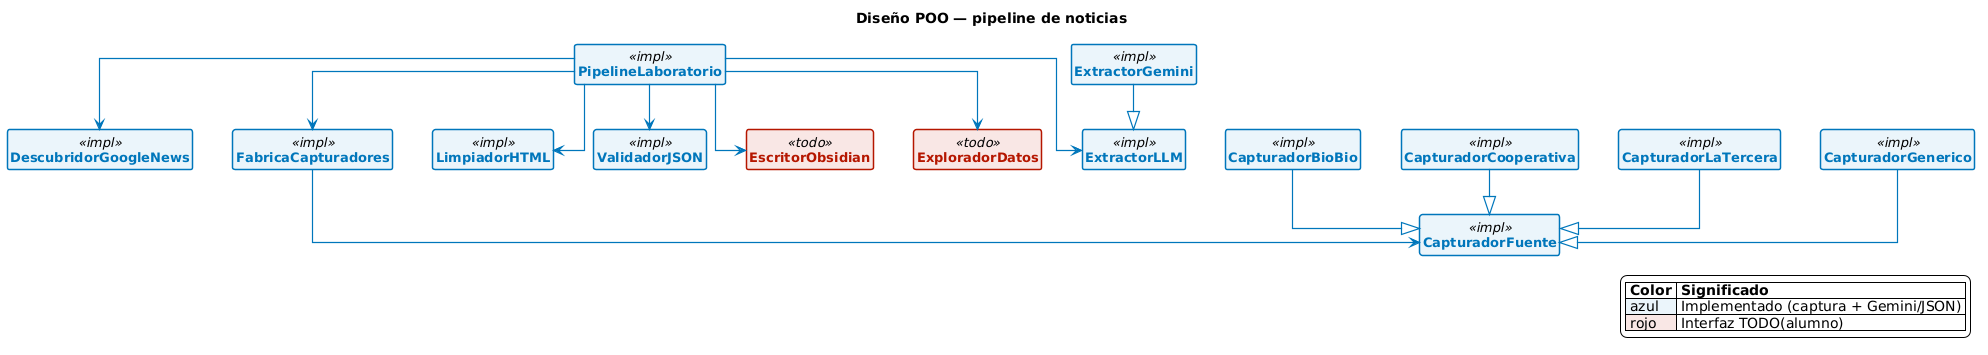
\includegraphics[width=0.98\linewidth,height=0.78\textheight,keepaspectratio]{diseno-poo.png}
\end{frame}

%================================================
\section{Puente: del texto al JSON}

%------------------------------------------------
\begin{frame}{De texto limpio al contrato de datos}
\small
El extractor \textbf{no descarga} la noticia otra vez. Lee \code{data/processed/\{id\}.txt} y debe devolver el mismo esquema en todas las noticias.

\vspace{0.2cm}
\begin{center}
\begin{tabular}{p{3.2cm}p{8.0cm}}
\toprule
\textbf{Campo} & \textbf{Rol} \\
\midrule
\code{id\_noticia} & Clave estable (N001, N002, \ldots). \\
\code{titulo}, \code{fecha}, \code{fuente}, \code{url} & Metadatos de la pieza. \\
\code{resumen} & Síntesis breve, sin inventar hechos. \\
\code{delitos}, \code{personas}, \code{lugares} & Entidades explícitas. \\
\code{relaciones} & Enlaces origen--tipo--destino. \\
\bottomrule
\end{tabular}
\end{center}

\begin{alertblock}<2->{Principio}
Si el dato no está en el texto, use \code{null} o una lista vacía. No complete con conocimiento previo del modelo.
\end{alertblock}
\end{frame}

%------------------------------------------------
\begin{frame}[fragile]{JSON esperado}
\tiny
\begin{lstlisting}
{
  "id_noticia": "N001",
  "titulo": "Operativo policial en La Serena",
  "fecha_publicacion": "2026-08-20",
  "fuente": "Medio de prensa",
  "url": "https://...",
  "resumen": "...",
  "delitos": ["Trafico de drogas"],
  "personas": [
    {"nombre": "Juan Perez", "rol": "imputado"}
  ],
  "organizaciones": ["Los X", "Carabineros"],
  "lugares": ["La Serena", "Region de Coquimbo"],
  "objetos": [
    {"tipo": "sustancia", "nombre": "cocaina", "cantidad": null, "unidad": null}
  ],
  "relaciones": [
    {"origen": "Juan Perez", "tipo": "INVESTIGADO_POR", "destino": "Trafico de drogas"}
  ]
}
\end{lstlisting}
\end{frame}

%================================================
\section{Extracción con Gemini}

%------------------------------------------------
\begin{frame}[fragile]{Clave API: nunca en el código}
\footnotesize
La clave se carga desde \code{.env} (excluido por \code{.gitignore}). El modelo por defecto es \code{gemini-2.0-flash}.

\vspace{0.15cm}
\begin{lstlisting}
cp .env.example .env
# edite .env y complete GEMINI_API_KEY
\end{lstlisting}

\vspace{0.1cm}
\begin{lstlisting}
# .env.example
GEMINI_API_KEY=
GEMINI_MODEL=gemini-2.0-flash
\end{lstlisting}

\scriptsize
\begin{alertblock}{Seguridad}
Si la clave aparece en GitHub, debe revocarla en Google AI Studio y generar otra. \code{src/config.py} lee las variables; no las hardcodee.
\end{alertblock}
\end{frame}

%------------------------------------------------
\begin{frame}[fragile]{Prompt estricto (código real)}
\tiny
\begin{lstlisting}[language=Python]
def construir_prompt(self, noticia: NoticiaFuente) -> str:
    campos = ", ".join(self.CAMPOS_OBLIGATORIOS)
    texto = (noticia.texto_limpio or "").strip()
    return (
        "Analiza la siguiente noticia delictual.\n\n"
        "Extrae solamente informacion explicita. No inventes datos.\n"
        "Devuelve exclusivamente JSON valido, sin markdown.\n\n"
        f"Campos obligatorios: {campos}.\n"
        "Si un dato no aparece, usa null o una lista vacia.\n\n"
        f"id_noticia: {noticia.id_noticia}\n"
        f"fuente: {noticia.fuente}\n"
        f"url: {noticia.url}\n\n"
        "NOTICIA:\n"
        f"{texto}\n"
    )
\end{lstlisting}

\scriptsize
El prompt viaja junto con el texto de \code{data/processed/}. Compare este esquema estricto con un prompt libre: el JSON será más estable.
\end{frame}

%------------------------------------------------
\begin{frame}[fragile]{Llamada a Gemini y guardado}
\tiny
\begin{lstlisting}[language=Python]
def extraer(self, noticia: NoticiaFuente) -> dict:
    if not GEMINI_API_KEY:
        raise RuntimeError("Falta GEMINI_API_KEY en .env")
    cliente = genai.Client(api_key=GEMINI_API_KEY)
    respuesta = cliente.models.generate_content(
        model=GEMINI_MODEL,
        contents=self.construir_prompt(noticia),
        config=types.GenerateContentConfig(
            automatic_function_calling=types.AutomaticFunctionCallingConfig(
                disable=True
            ),
            response_mime_type="application/json",
            temperature=0,
        ),
    )
    data = self._parsear_json(respuesta.text)
    data["id_noticia"] = noticia.id_noticia   # no dejar que el modelo lo cambie
    ruta = DIR_JSON / f"{noticia.id_noticia}.json"
    ruta.write_text(json.dumps(data, ensure_ascii=False, indent=2))
    return data
\end{lstlisting}

\scriptsize
\begin{block}{Parseo}
Gemini a veces envuelve el JSON en un bloque markdown. \code{\_parsear\_json} quita esos fences antes de \code{json.loads}.
\end{block}
\end{frame}

%------------------------------------------------
\begin{frame}{Flujo de \texttt{python main.py extraer}}
\centering
\resizebox{0.92\linewidth}{!}{%
\begin{tikzpicture}[font=\scriptsize, node distance=0.55cm,
box/.style={draw=blue, fill=lightblue, rounded corners=2mm, minimum width=2.4cm, minimum height=0.7cm, align=center},
arrow/.style={-{Latex[length=1.7mm]}, thick, blue}]
\node[box] (a) {urls.csv};
\node[box, right=0.5cm of a] (b) {processed\\N00X.txt};
\node[box, right=0.5cm of b] (c) {ExtractorGemini};
\node[box, below=0.7cm of c] (d) {json/N00X.json};
\node[box, left=0.5cm of d] (e) {ValidadorJSON};
\node[draw=red, fill=red!10, rounded corners=2mm, minimum width=2.4cm, minimum height=0.7cm, align=center, left=0.5cm of e] (f) {Obsidian\\TODO};
\draw[arrow] (a)--(b);
\draw[arrow] (b)--(c);
\draw[arrow] (c)--(d);
\draw[arrow] (d)--(e);
\draw[-{Latex[length=1.7mm]}, thick, red] (e)--(f);
\end{tikzpicture}%
}

\vspace{0.35cm}
\footnotesize
Una noticia con JSON inválido o error de API \textbf{no tumba el lote}: se registra el fallo y se continúa (igual que en la captura).
\end{frame}

%------------------------------------------------
\begin{frame}[fragile]{Validación: el LLM no es la fuente de verdad}
\tiny
\begin{lstlisting}[language=Python]
class ValidadorJSON:
    CAMPOS_OBLIGATORIOS = [
        "id_noticia", "titulo", "fecha_publicacion", "fuente", "url",
        "resumen", "delitos", "personas", "organizaciones",
        "lugares", "objetos", "relaciones"
    ]
    CAMPOS_LISTA = ["delitos", "personas", "organizaciones",
                    "lugares", "objetos", "relaciones"]

    def validar(self, ruta):
        data = json.loads(Path(ruta).read_text(encoding="utf-8"))
        faltantes = [c for c in self.CAMPOS_OBLIGATORIOS if c not in data]
        if faltantes:
            raise ValueError(f"faltan campos {faltantes}")
        for campo in self.CAMPOS_LISTA:
            if not isinstance(data[campo], list):
                raise ValueError(f"'{campo}' debe ser una lista")
        return data
\end{lstlisting}

\scriptsize
Implementación mínima. \todo{}: registrar nulos, tipos incorrectos y cobertura para Data Understanding.
\end{frame}

%------------------------------------------------
\begin{frame}[fragile]{Cómo ejecutar la extracción}
\tiny
\begin{lstlisting}
conda activate lab-noticias-obsidian
cp .env.example .env          # una sola vez; complete GEMINI_API_KEY
python main.py capturar       # si aún no hay data/processed/*.txt
python main.py extraer        # llama a Gemini y valida cada JSON
\end{lstlisting}

\vspace{0.15cm}
\scriptsize
Salida esperada (resumida):
\begin{lstlisting}
== Etapa: extraer (Gemini) ==
  [N001] BioBioChile
    OK: JSON validado
  [N002] Cooperativa
    OK: JSON validado
Extraccion finalizada: 4 ok, 0 fallos, 4 total
\end{lstlisting}

\footnotesize
Los archivos quedan en \code{data/json/N00X.json}. Sin clave, el programa se detiene con un mensaje claro (no un traceback opaco).
\end{frame}

%------------------------------------------------
\begin{frame}{Qué puede mejorar el alumno (Gemini ya corre)}
\small
El extractor es didáctico, no de producción. Mejoras sugeridas:

\vspace{0.15cm}
\begin{itemize}
\item Reintentos con espera ante HTTP 429 o timeouts.
\item Recorte de textos muy largos antes del prompt.
\item Verificar tipos internos (\code{personas[].nombre}, \code{relaciones[].tipo}).
\end{itemize}

\begin{block}{Criterio}
Mejorar no significa reescribir el módulo desde cero. Significa endurecer el contrato sin romper \code{python main.py extraer}.
\end{block}
\end{frame}

%================================================
\section{Obsidian: tarea del alumno}

%------------------------------------------------
\begin{frame}{Obsidian como persistencia}
\small
\begin{itemize}[<+->]
\item No se usará SQLite, MongoDB ni Neo4j.
\item La persistencia final serán archivos Markdown enlazados.
\item Cada noticia y cada entidad relevante tendrá su propia nota.
\item Las relaciones se expresan con \code{[[wiki-links]]} y se ven en el grafo de Obsidian.
\end{itemize}

\begin{alertblock}<5->{Cambio clave}
El sistema no guarda filas en una base de datos. Guarda conocimiento como una red de notas conectadas.
\end{alertblock}
\end{frame}

%------------------------------------------------
\begin{frame}[fragile]{Jerarquía del vault}
\footnotesize
\begin{block}{Estructura esperada}
\ttfamily\tiny
obsidian\_vault/\\
|-- 00\_Indice.md\\
|-- Noticias/\\
|   |-- N001.md\\
|   |-- N002.md\\
|   `-- N003.md\\
|-- Delitos/\\
|   |-- Trafico\_de\_drogas.md\\
|   `-- Homicidio.md\\
|-- Personas/\\
|-- Organizaciones/\\
|-- Lugares/\\
|-- Objetos/\\
`-- Relaciones/\\
\end{block}

\scriptsize
Las carpetas ya existen (con \code{.gitkeep}). El alumno debe generar los \code{.md}. La estructura es parte del resultado evaluado.
\end{frame}

%------------------------------------------------
\begin{frame}[fragile]{Nota Markdown de una noticia}
\tiny
\begin{lstlisting}
---
id: N001
fecha_publicacion: 2026-08-20
fuente: Medio de prensa
url: https://...
---

# Operativo policial en La Serena

## Resumen
Texto breve generado desde el JSON.

## Delitos
- [[Trafico de drogas]]

## Personas
- [[Juan Perez]] - imputado

## Lugares
- [[La Serena]]

## Relaciones
- [[Juan Perez]] -- INVESTIGADO_POR --> [[Trafico de drogas]]
\end{lstlisting}
\end{frame}

%------------------------------------------------
\begin{frame}{Notas de entidades}
\small
Además de las noticias, el laboratorio debe generar una nota por entidad.

\vspace{0.2cm}
\begin{columns}[T,onlytextwidth]
\column{0.47\textwidth}
\begin{block}{Ejemplo: Delito}
\scriptsize
\code{Delitos/Trafico\_de\_drogas.md}
\begin{itemize}
\item Noticias relacionadas.
\item Personas asociadas.
\item Organizaciones mencionadas.
\item Lugares donde aparece.
\end{itemize}
\end{block}
\column{0.47\textwidth}
\begin{alertblock}{Ejemplo: Persona}
\scriptsize
\code{Personas/Juan\_Perez.md}
\begin{itemize}
\item Noticias donde aparece.
\item Rol observado.
\item Delitos asociados.
\item Organizaciones relacionadas.
\end{itemize}
\end{alertblock}
\end{columns}
\end{frame}

%------------------------------------------------
\begin{frame}[fragile]{Nombres de archivo y \texttt{slugify}}
\tiny
\begin{lstlisting}[language=Python]
# Ya implementado en src/conocimiento/utilidades.py
def slugify(text):
    text = unicodedata.normalize("NFKD", text)
    text = "".join(c for c in text if not unicodedata.combining(c))
    text = re.sub(r"[^a-zA-Z0-9]+", "_", text)
    return text.strip("_") or "sin_nombre"

slugify("Tráfico de drogas")       # Trafico_de_drogas
enlace_obsidian("Juan Perez")      # [[Juan Perez]]
\end{lstlisting}

\scriptsize
\begin{block}{Motivo}
Los nombres deben ser estables para que los enlaces de Obsidian no se rompan. Use estas funciones en \code{EscritorVaultObsidian}.
\end{block}
\end{frame}

%------------------------------------------------
\begin{frame}[fragile]{Índices de entidades (idea de implementación)}
\tiny
\begin{lstlisting}[language=Python]
from collections import defaultdict

indice_delitos = defaultdict(set)
indice_personas = defaultdict(set)
indice_lugares = defaultdict(set)

for data in noticias_json:
    nid = data["id_noticia"]
    for delito in data["delitos"]:
        indice_delitos[delito].add(nid)
    for persona in data["personas"]:
        indice_personas[persona["nombre"]].add(nid)
    for lugar in data["lugares"]:
        indice_lugares[lugar].add(nid)
\end{lstlisting}

\scriptsize
Incorpore este patrón en \code{escribir\_entidades}: una nota por entidad con la lista de noticias relacionadas.
\end{frame}

%------------------------------------------------
\begin{frame}[fragile]{Interfaz que el alumno debe completar}
\tiny
\begin{lstlisting}[language=Python]
class EscritorVaultObsidian(EscritorObsidian):
    def escribir_noticia(self, data: dict) -> Path:
        # TODO(alumno): plantilla Markdown con YAML y [[enlaces]]
        raise EtapaPendienteAlumno(...)

    def escribir_entidades(self, noticias: list[dict]) -> None:
        # TODO(alumno): una nota por delito, persona, lugar, ...
        raise EtapaPendienteAlumno(...)

    def escribir_indice(self, noticias: list[dict]) -> Path:
        # TODO(alumno): obsidian_vault/00_Indice.md
        raise EtapaPendienteAlumno(...)

    def escribir_vault(self, noticias: list[dict]) -> None:
        # TODO(alumno): orquestar los tres metodos anteriores
        raise EtapaPendienteAlumno(...)
\end{lstlisting}
\end{frame}

%------------------------------------------------
\begin{frame}[fragile]{Cómo ejecutar Obsidian (cuando lo implemente)}
\tiny
\begin{lstlisting}
python main.py extraer      # genera data/json/*.json
python main.py obsidian     # debe leer esos JSON y escribir el vault
\end{lstlisting}

\vspace{0.15cm}
\footnotesize
Hoy, sin completar la clase, verá una pista \todo{} y el programa no falla en silencio.

\vspace{0.2cm}
Puede empezar \textbf{sin} llamar a Gemini: hay un fixture didáctico en \code{data/json/ejemplo\_N001.json} con el esquema de las slides. Úselo para probar plantillas Markdown.

\vspace{0.15cm}
Después de implementar, abra la carpeta \code{obsidian\_vault/} como bóveda en Obsidian y revise el grafo.
\end{frame}

%------------------------------------------------
\begin{frame}{Relaciones y agrupamientos simples}
\small
\begin{itemize}[<+->]
\item Un grupo de noticias puede formarse porque comparte el mismo tipo de delito.
\item También puede formarse porque comparte una persona, organización o comuna.
\item Obsidian permite visualizar esas conexiones sin entrenar un algoritmo de clustering.
\end{itemize}

\begin{center}
\resizebox{0.72\linewidth}{!}{%
\begin{tikzpicture}[font=\scriptsize]
\node[draw=red, fill=red!10, rounded corners=2mm] (d) at (0,0) {Tráfico de drogas};
\node[draw=blue, fill=lightblue, rounded corners=2mm] (n1) at (-3.2,1.0) {N001};
\node[draw=blue, fill=lightblue, rounded corners=2mm] (n2) at (-3.2,-1.0) {N007};
\node[draw=blue, fill=lightblue, rounded corners=2mm] (n3) at (3.2,0) {N015};
\draw[-{Latex[length=1.6mm]}, thick, blue] (n1)--(d);
\draw[-{Latex[length=1.6mm]}, thick, blue] (n2)--(d);
\draw[-{Latex[length=1.6mm]}, thick, blue] (n3)--(d);
\end{tikzpicture}%
}
\end{center}
\end{frame}

%================================================
\section{Cierre}

%------------------------------------------------
\begin{frame}[fragile]{Comandos del orquestador}
\tiny
\begin{lstlisting}
python main.py descubrir   # Google News RSS -> data/urls.csv
python main.py capturar    # URLs -> data/raw + data/processed
python main.py extraer     # Gemini -> data/json (requiere GEMINI_API_KEY)
python main.py obsidian    # TODO(alumno) vault Markdown
python main.py analizar    # TODO(alumno) Data Understanding
python main.py pipeline    # descubrir + capturar + extraer; avisa pendientes
\end{lstlisting}

\scriptsize
Secuencia de esta entrega: \code{capturar} $\rightarrow$ \code{extraer} $\rightarrow$ (alumno) \code{obsidian}.
\end{frame}

%------------------------------------------------
\begin{frame}{Ética y uso responsable}
\small
\begin{itemize}
\item Extraiga solo lo \textbf{explícito} en la noticia. No infiera culpabilidad.
\item Los roles (detenido, imputado, acusado, condenado, víctima, testigo) \textbf{no son equivalentes}.
\item Conserve la URL y cite la fuente en cada nota de Obsidian.
\item No suba \code{.env} ni claves a GitHub.
\item Uso académico de la API y de los sitios de prensa: no sobrecargue servidores.
\end{itemize}
\end{frame}

%------------------------------------------------
\begin{frame}{Errores comunes}
\scriptsize
\begin{center}
\begin{tabular}{p{5.4cm}p{6.6cm}}
\toprule
\textbf{Síntoma} & \textbf{Qué revisar} \\
\midrule
Falta \code{GEMINI\_API\_KEY} & Copiar \code{.env.example} a \code{.env}. \\
JSON envuelto en markdown & El parseo ya quita fences; si falla, endurezca el prompt. \\
Campos faltantes & \code{ValidadorJSON} lanza \code{ValueError}. \\
Una noticia tumba el lote & No debería: el pipeline continúa. \\
Vault vacío o sin enlaces & Completar \code{EscritorVaultObsidian} y usar \code{slugify}. \\
Clave en el historial de Git & Revocar y generar otra en AI Studio. \\
\bottomrule
\end{tabular}
\end{center}
\end{frame}

%------------------------------------------------
\begin{frame}{Secuencia sugerida de trabajo}
\scriptsize
\begin{enumerate}[<+->]
\item Activar conda y completar \code{.env} con \code{GEMINI\_API\_KEY}.
\item Verificar captura: \code{python main.py capturar}.
\item Ejecutar \code{python main.py extraer} y abrir un JSON en \code{data/json/}.
\item Mejorar prompt o validación si el JSON es ruidoso.
\item Completar \code{EscritorVaultObsidian} (puede partir de \code{ejemplo\_N001.json}).
\item Ejecutar \code{python main.py obsidian} y abrir el vault.
\item Corregir nombres inconsistentes y enlaces rotos.
\item Completar \code{ExploradorDatos} (siguiente etapa).
\end{enumerate}
\end{frame}

%------------------------------------------------
\begin{frame}{Cierre}
\begin{columns}[T,onlytextwidth]
\column{0.58\textwidth}
\small
\begin{itemize}[<+->]
\item El lab 01 entregó texto limpio y reproducible.
\item Esta parte convierte ese texto en JSON validado con Gemini.
\item El LLM estructura, pero no reemplaza la validación humana.
\item El valor final está en el grafo de Obsidian que el alumno debe construir.
\end{itemize}
\column{0.36\textwidth}
\centering
\resizebox{\linewidth}{!}{%
\begin{tikzpicture}[every node/.style={font=\tiny}]
\node[draw=blue, rounded corners=2mm, fill=lightblue, minimum width=2.7cm, minimum height=0.55cm] (t1) at (0,1.5) {Texto no estructurado};
\node[draw=blue, rounded corners=2mm, fill=white, minimum width=2.7cm, minimum height=0.55cm] (t2) at (0,0.2) {JSON validado};
\node[draw=red, rounded corners=2mm, fill=red!8, minimum width=2.7cm, minimum height=0.55cm] (t3) at (0,-1.1) {Grafo en Obsidian};
\draw[-{Latex[length=1.8mm]}, thick, blue] (t1)--(t2);
\draw[-{Latex[length=1.8mm]}, thick, red] (t2)--(t3);
\end{tikzpicture}%
}
\end{columns}
\end{frame}

%------------------------------------------------
\begin{frame}
\centering
\Huge ¿Preguntas?
\end{frame}

\end{document}
